\chapter{Knihovna publicvfk}
\label{4-plugin}
Tato kapitola je věnována informacím o nové knihovně
%% ML: v textu Vam chybi obecne provazanost (napr. zde chybi odkaz na
%% kapitolu QGIS VFK Plugin)
\textbf{publicvfk} pro zásuvný modul \textit{QGIS VFK Plugin} a její
%% ML: ve vete mate dvakrat souslovi ``zasuvny modul'', zkuste prepsat
integraci do zásuvného modulu. Je popsána funkčnost knihovny, uvedeno
%% ML: druhou cast vety prepiste, zni sroubovane. - napr. knihovny
%% jeji vstupy a vystupy.
co je pro knihovnu vstupem a co výstupem. Poté je představena ukázka
funkčnosti na testovacích datech a popsány podrobnosti o způsobu
integrace do výše zmíněného zásuvného modulu \textit{QGIS VFK
 %% ML: tvorbu ceho? textu?
  Plugin}. Pro tvorbu je čerpáno ze zdrojů \cite{cookbook,
  ucebnicepython}.

\section{Funkčnost knihovny}
\label{sec:funknost_knihovny}
Knihovna načítá pomocí VFK driveru knihovny GDAL (viz
%% ML: cimz? nejasna veta, zkuste preformulovat
kap. \ref{subsec:gdal_vfk}) textový soubor ve formátu \zk{VFK}, čímž
%% ML: SQL -> SQLite
vznikne \zk{SQL} databáze s načtenými daty. \zk{VFK} soubor již není
%% ML: SQL -> SQLite
dále využíván, knihovna místo toho přistupuje k vytvořené \zk{SQL}
databázi. Následně je zkontrolována verze knihovny
GDAL[\ref{sec:gdal}]. Pokud není vyšší než 2.2, tak musí být proveden
%% ML: prikaz nemate vysvetlen, co dela? - napr. v poznamce pod carou
příkaz \verb|self.dsn_vfk.GetLayerByName('HP').GetFeature(1)|, který
se postará o sestavení geometrie všech datových bloků souvisejících s
blokem hranic parcel (HP)[\ref{sec:sestaveni_geometrie}].

%% ML: nacitani dat z databaze (v GDAL 2.2 je to opet jiz vyreseno)
Pro správné fungování při načítání dat je nezbytné přidat do databáze
tabulku geometrie (\verb|geometry columns|) a tabulku souřadnicového
systému (\verb|spatial_ref_sys|). Dojde tak k vytvoření prostorové
databáze\footnote{Databáze ukládající prostorovou složku dat.}. SQLite
%% ML: bez techto takulek?
%% ML: nez o datovem typu bych hovoril o typu prvku/geometrie
driver knihovny GDAL bez tabulek není schopen rozeznat datový typ vrstev. U novější
%% ML: GDAL 2.2
verze knihovny dochází k vytvoření tabulek automaticky.

%% ML: nemate uplne vysvetleno, proc je nacitani nutne provadet pomoci
%% SQLite driveru. VFK driver totiz take cte data z databaze (ale
%% neuvidi bloky PAR a BUD jelikoz chybi v podkladovem VFK souboru)

Po vytvoření prostorové databáze následují postupně kroky, během
kterých vznikají data v připojené databázi:
\begin{enumerate}[leftmargin=50pt]
\item Vytvoření tabulky s názvem PAR pro parcely
\item Sestavení a zapsání geometrie parcel i s atributy
\item Vytvoření tabulky s názvem BUD pro budovy
\item Sestavení a zapsání geometrie budov včetně atributů
\end{enumerate}

Pro sestavení geometrie parcel je využito datového bloku HP (hranice
parcel), kde je možné pomocí atributů \verb|PAR_ID_1| a
\verb|PAR_ID_2| (viz kap. \ref{subsec:bloky_par_bud}) zjistit unikátní seznam
%% ML: cisel -> identifikatoru
čísel všech parcel. Pro každou parcelu jsou následně nalezeny
%% ML: geometrie sestavena geometrickou cestou? zkuste preformulovat
příslušné hranice. Samotná geometrie parcel je sestavená geometrickou
%% ML: veta nedava smysl, prepiste
cestou, tedy postupným spojováním navazujících hranici parcelu po
parcele. Následující pseudokód(\ref{alg:sestaveni_parcely}) popisuje
proces sestavení a uložení geometrie parcel. Na řádku 10 je volána
metoda \verb|build_bound()|(viz kap. \ref{subsec:sestaveni_geometrie}), která
provádí sestavení geometrie z příslušných hranic. Princip metody je
podrobněji znázorněn diagramem v příloze \ref{fig:logika_geometrie}.

\begin{algorithm}
\caption{Logika sestavení a uložení geometrie parcel}
\label{alg:sestaveni_parcely}
	\begin{algorithmic}[1]
	\STATE{číslaParcel = zjisti SQL příkazem unikátní čísla parcel}
	\STATE{NeuzavřenéParcely = prázdný seznam}
	\STATE{Začátek transakce}
	\FOR{Parcela \textbf{in} číslaParcel}
		\STATE{seznamGeometriíHranice = prázdný seznam}
		\FOR{prvek \textbf{in} filtrVrstvy(vrstva = HraniceParcel, filtr = Parcela)}
			\STATE{geometrie = geometrie prvku}
			\STATE{přidej geometrie do seznamGeometriíHranice}
		\ENDFOR
		\STATE{polygonGeometrie = sestav geometrii ze seznamGeometriíHranice}
		\IF{polygonGeometrie \textbf{is not} prázdný}
			\STATE{převeď polygonGeometrie do roviny(2D)}
		\ELSE
			\STATE{Přidej číslo parcely do NeuzavřenéParcely}
		\ENDIF
		\STATE{Vytvoř nový řádek tabulky}
		\STATE{Nastav geometrii sestavované parcely do nového řádku}
		\STATE{Nastav hodnotu do sloupce \verb|"id_par"| pro nový řádek}
		\STATE{Nastav hodnotu do sloupců \verb|"kmenove_cislo_par"|, \verb|"poddeleni_cisla_par"| pro nový řádek}
		\STATE{Přidej nově vytvořený řádek do tabulky}
	\ENDFOR
	\STATE{Konec transakce}
	\end{algorithmic}
\end{algorithm}

K sestavení geometrie budov je využito datového bloku SBP (spojení
bodů polohopisu) a bloku OB (obrazy budov). Nejprve jsou zjištěna z
bloku OB unikátní identifikační čísla budov včetně příslušných
identifikačních čísel hranic budov, pro které je následně vyhledána
geometrie v tabulce SBP. Sestavení geometrie budov probíhá také
geometrickou cestou. Logika sestavování geometrie je stejná jako v
případě parcel, viz příloha \ref{fig:logika_geometrie}.
%zdroj: http://gdal.org/drv_sqlite.html

\section{Vstupní data}
Vstupními daty je pro knihovnu textový soubor ve formátu \zk{VFK} s
neúplnými daty (viz kap. \ref{subsec:neuplna_data}). Knihovna přebírá
%% ML: adresa -> cesta
adresu vstupního souboru, dochází k načtení dat VFK
driverem (viz kap. \ref{subsec:gdal_vfk}) a zápisu do databáze.

\subsection{Testovací data}
Zkomprimovaná testovací data ve formátu \zk{VFK} byla stažena pro
katastrální území Abertamy na adrese:
\href{http://services.cuzk.cz/vfk/ku/20170901/600016.zip}{http://services.cuzk.cz/vfk/ku/20170901/600016.zip}.
     {\scriptsize
\begin{lstlisting}[caption=Ukázka bloku hranic parcel(HP) -- definice bloků a věty dat(zdroj:vlastní), label=lst:data]
&BHP;ID N30;STAV_DAT N2;DATUM_VZNIKU D;DATUM_ZANIKU D;PRIZNAK_KONTEXTU N1;
RIZENI_ID_VZNIKU N30;RIZENI_ID_ZANIKU N30;TYPPPD_KOD N10;PAR_ID_1 N30;PAR_ID_2 N30
&DHP;3491827403;0;"07.04.2009 08:59:39";"";3;1991606403;;21900;706860403;708070403 
&DHP;3491828403;0;"07.04.2009 08:59:39";"";3;1991606403;;21900;706860403;708070403
&DHP;3491829403;0;"07.04.2009 08:59:39";"";3;1991606403;;21900;706860403;708070403
&DHP;3491830403;0;"07.04.2009 08:59:39";"";3;1991606403;;21900;706860403;708070403
&DHP;3491831403;0;"07.04.2009 08:59:39";"";3;1991606403;;21900;706860403;708070403
\end{lstlisting}}
Na řádcích 1-2~(\ref{lst:data}) je rozdělený uvozovací řádek datového
bloku HP (hranic parcel). Řádky 3-7~(\ref{lst:data}) představují věty
%% ML: poradi datovych vet je v podstate nahodne, je dano exportem z
%% publikacni DB ISKN, ale to pouze na okraj
dat, ve kterých jsou uložena vlastní data ve stanoveném pořadí.

%% ML: Overereni funkcnosti knihovny?
\subsection{Funkčnost knihovny s testovacími daty}

%% ML: prvni veta nedava smysl, databaze neni prostorova (chybi geometry_columns)
%% ML: take nekde chybi prikaz, ktery by ukazoval jak tato DB vznikla (ogrinfo file.vfk)
Přestože databáze obsahuje datové vrstvy, tak SQLite driver není schopen
%% ML: coz je v poradku, jelikoz vstupni data tyto bloky neobsahovala
vrstvy rozeznat, proto mají všechny hodnotu None. Zároveň databáze
neobsahuje bloky parcel a budov.
\begin{figure}[H]
	 \centering
      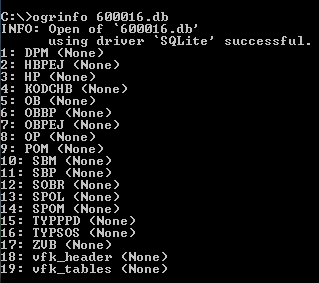
\includegraphics[height=5cm]{./pictures/funkcnost_knihovny_pred.png}
      \caption{Databáze před použitím knihovny (zdroj:vlastní)}
      \label{fig:funkcnost_pred}
\end{figure}

%% ML: driver se jmenuje SQLite (casta chyba v textu)
Po použití knihovny \textbf{publicvfk} SQL driver datové bloky již
rozezná díky přidaným tabulkám geometrie a souřadnicového systému. V
databázi jsou nyní obsaženy sestavené bloky parcel
\textbf{PAR (Polygon)} a budov \textbf{BUD (Polygon)}.
\begin{figure}[H]
	 \centering
     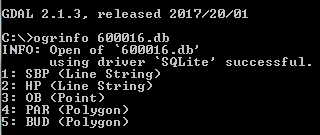
\includegraphics[height=3cm]{./pictures/funkcnost_knihovny_po.png}
     \caption{Databáze po použití knihovny(zdroj:vlastní)}
     \label{fig:funkcnost_po}
\end{figure}  
  
\section{Výstupní data}
Výstupem knihovny je sestavená geometrie bloků parcel a
budov. Geometrie je společně s atributy zapsána do VFK
driverem (viz kap. \ref{subsec:gdal_vfk}) vytvořené databáze.

\section{Popis tříd knihovny a jejich metod}
\label{sec:popis_trid}
V následující podkapitole jsou představeny jednotlivé třídy knihovny,
jejich členské metody a popsáno, co která třída a metoda obstarává.

\subsection{VFKBuilderError}
Tato třída dědí vlastnosti třídy Exception a je volána v případě, že
%% ML: zadne jine pripadne chybove stavy neexistuji?
nastane chyba. To se může stát není-li připojen \zk{VFK} soubor nebo
databáze.
\subsection{VFKBuilder}
\label{subsec:sestaveni_geometrie}
Mateřská třída, která obsahuje společné metody tříd
\textit{VFKParBuilder} a \textit{VFKBudBuilder} určených pro sestavení
geometrie parcel i budov.
\begin{itemize}[leftmargin=50pt]
\item \verb|__init__()|

%% ML: preteceni textu v radku
V konstruktoru třídy dochází k vytvoření tabulky geometrie
(\verb|geometry columns|) a tabulky souřadnicového systému
(\verb|spatial_ref_sys|), bez kterých by nebylo možné číst geometrii z
databáze. V případě nepřipojeného zdroje dat - \zk{VFK} souboru, je
%% ML: trida neni volana, je vyvolana vyjimka, ktera je obslouzena tridou...
volána třída VFKBuilderError a zobrazena chybová hláška.
\item \verb|build_bound()|

Hlavní metoda, která sestavuje geometrii jednotlivých hranic. V
%% ML: hranice s dirami, nemel jste na mysli polygon?
případě hranice s dírami dojde k vytvoří seznamu s více geometriemi,
%% ML: nejdelsi ? nejvetsi vymera ?
ve kterém je nalezena největší a ze zbylých geometrií jsou vytvořeny
díry. Sestavení probíhá geometrickou cestou. Nejdříve je přidána první
hranice, poté hranice obsahující koncový bod první hranice a tak
%% ML: tady by se hodil odkaz na pseudokod
dokola. Na závěr je otestováno uzavření všech hranic v seznamu
geometrií (první bod hranice je shodný s posledním bodem hranice). Pro
názornost principu metody je v příloze vytvořen
diagram \ref{fig:logika_geometrie}.
\item \verb|add_boundary()|

Metoda pro přidávání jedné hranice do geometrie. Přidávání hranice
probíhá bod po bodu a přidaná hranice je ze seznamu hranic odstraněna,
aby se seznam zmenšil. Všechny hranice nemají stejnou
orientaci (některé na sebe navazují koncovými body), tudíž je potřeba
%% ML: v nekterych pripadech
body hranice přidávat "odzadu".
\item \verb|filter_layer()|

Na základě specifikovaného atributového filtru a názvu datového bloku
vrací výsledné hodnoty uložené v seznamu.
\item \verb|executeSQL()|

Provádí \zk{SQL} dotaz v databázi a vrací výsledek uložený do seznamu.

\end{itemize}
\subsection{VFKBudBuilder}
Potomek třídy \textbf{VFKBuilder}. Třída sestavuje geometrii budov a
ukládá ji do nově vytvořené tabulky BUD v databázi. Ukládání probíhá v
transakci.
\begin{itemize}[leftmargin=50pt]
\item \verb|__init__()|

Konstruktor třídy, kde je vytvořena nová tabulka pro budovy -- BUD a~atribut \verb|id_bud|.
\item \verb|build_all_bud()|

 %% ML: preformulovat, prvni veta je matouci
Metoda se stará o sestavení všech nebo jen části všech budov. To je
možné nastavit parametrem limit. Po sestavení probíhá v transakci
uložení geo\-metrií a atributů do tabulky BUD v databázi.
\end{itemize}
\subsection{VFKParBuilder}
Potomek třídy \textbf{VFKBuillder}. Zde dochází k vlastnímu sestavení
geometrie parcel, vytvoření nové tabulky PAR v databázi a zapsání
dat. Zapisuje se identifikační číslo parcely (\verb|par_id|), kmenové
číslo parcely (\verb|kmenove_cislo_par|), poddělení čísla
parcely (\verb|poddeleni_cisla_par|) a hlavně geometrie dané
parcely. Zápis do databáze je proveden v transakci, čímž je zaručené
korektní zapsání všech parcel.

\begin{itemize}[leftmargin=50pt]
\item \verb|__init__()|

Konstruktor třídy, kde je vytvořena nová tabulka pro parcely -- PAR včetně atributů.
\item \verb|build_all_par()|

Zde probíhá samotné sestavení všech parcel. Po sestavení je parcela
uložena do databáze i s příslušnými atributy. Metodě je možné nastavit
%% ML: Zakladne?
kolik parcel má sestavit. Základně dochází k sestavení všech parcel.

\end{itemize}
\section{Integrace knihovny do zásuvného modulu}
\label{sec:integrace_knihovny}

%% ML: zkuste prvni vetu preformulovat, nezni dobre
Základem integrace je správné umístění do kódu zásuvného modulu,
přesněji do souboru \textit{mainApp.py}. Je potřeba zachovat
%% ML: zpoplatnenych a verejne dostupnych - pripadne upravit i dale v
%% textu (ani zpoplatnena data nejsou uplna...)
funkcionalitu při otevření úplných i neúplných dat. Jsou-li data
úplná, funguje zásuvný modul standardně. Pokud jsou data neúplná --
%% ML: pouziti trid ? zavolani neni korektni termin
neobsahují bloky PAR a BUD, dojde k jejich sestavení a tedy zavolání
třídy z nově integrované knihovny \textbf{publicvfk}.

Nejdříve je knihovna pomocí metody import nahrána. Poté je ve funkci
\textbf{loadVfkFile()} proveden test na přítomnost bloku parcel('PAR')
pomocí metody GetLayerName():
\begin{lstlisting}[language=Python, numbers=none]
t_par = self.__mOgrDataSource.GetLayerByName('PAR')
\end{lstlisting}
Předpokladem je, že bloky parcel a budov jsou v datech obsaženy buďto oba nebo žádný, proto je testována jen přítomnost bloku parcel. Není-li blok obsažen, dojde k uzavření zdroje dat:
\begin{lstlisting}[language=Python, numbers=none]
self.__mOgrDataSource = None
\end{lstlisting}
, aby mohlo proběhnout sestavení bloků parcel a budov. Knihovna si
vytváří vlastní připojení k \zk{VFK} souboru a databázi, proto je
třeba zdroj dat uzavřít a předejít tak zdvojenému připojení k \zk{VFK}
souboru či databázi. Vícenásobné připojení může způsobit chybu. Poté
%% ML: neobsazenych je kostrbate slovo
následuje samotné sestavení neobsažených bloků parcel a budov. Za
%% ML: odkaz na kapitoly popisujici tridy?
sestavení parcel zodpovídá třída \textit{VFKParBuilder} a o sestavení
%% ML: neni to jiz jasne, navic pokud umistite odkaz na popis trid,
%% tak o to bude cela vec jasnejsi
budov třída \textit{VFKBudBuilder}, obě třídy jsou z integrované
knihovny. Nejprve jsou deklarovány objekty dané třídy a následně jsou
volány metody příslušných tříd pro sestavení geometrií:

\begin{lstlisting}[language=Python, numbers=none]
# Build Parcels
parcels = VFKParBuilder(fileName)
parcels.build_all_par()
# Build Buildings
buildings = VFKBudBuilder(fileName)
buildings.build_all_bud()
\end{lstlisting}

Po ukončení sestavování bloků parcel a budov je zdroj dat pomocí
%% ML: nepiste, kde konkteretne DB vznika, to se stejne muze zmenit,
%% pouze muzete zminit, ze plugin pouziva vlastni nastaveni pro DB
%% tak, aby byl schopen nahrat vice VFK soubor ci zpracovat zmenove
%% soubory
proměnné prostředí nastaven na databázi, která vznikne o adresář výš
při otevření \zk{VFK} souboru a nese jméno \zk{VFK} souboru, kde je
místo přípony \verb|.vfk| přípona \verb|_stav.db|: {\small
\begin{lstlisting}[language=Python, numbers=none]
self.__mOgrDataSource = ogr.Open(os.environ['OGR_VFK_DB_NAME'], 0)
self.__mDataSourceName = os.environ['OGR_VFK_DB_NAME']
\end{lstlisting}}
%self.__mDataSourceName = os.environ['OGR_VFK_DB_NAME'] PROČ,k čemu proměnná je? nastavuje zde taky prostredi? 

V této databázi jsou uložena data z načtení \zk{VFK} souboru a také
knihovnou vytvořené tabulky s bloky PAR a BUD. Zásuvný modul z této
databáze čerpá data, která po načtení vizualizuje v mapovém okně.

Při načítání neúplných dat \zk{VFK} může nastat situace, kdy už jsou
tabulky parcel a budov nebo jen jednoho bloku v databázi
zapsané. SQLite driver však bloky nedokáže rozeznat, protože databáze
není prostorová (viz kap. \ref{sec:funknost_knihovny}). Pro tento
případ je v knihovně před vytvářením jednotlivé tabulky testováno,
jestli databáze blok parcel nebo budov opravdu neobsahuje. Tento test
je v kódu umístěn až za vložením tabulek s geometrií a souřadnicovým
systémem, tudíž je nepřítomnost zapsaných dat vyloučena. Zjistí-li se
po přidání tabulek, že jsou oba datové bloky -- parcely a budovy v
databázi již zapsané, knihovna nové sestavení neprovádí.

\section{Testování knihovny}

Funkčnost knihovny je možné otestovat z příkazové řádky. K testování
%% ML: Ta veta je zavadejici, k testovani neni pouzit sys modul, pres
%% sys.argv jste pouze schopen zjisit parametry pri spusteni skriptu
je využit modul sys, který je obsažen v základní distribuci Pythonu a
díky kterému je možné realizovat množství úloh spojených s
interpretrem. Příkaz pro spuštění se skládá z názvu knihovny a
\zk{VFK} souboru včetně přípony, oddělených mezerou. Například:
\textit{python publicvfk.py 600016.vfk} (viz
kap. \ref{fig:testovani_ukazka}). Jméno knihovny a další argumenty
(v~našem případě pouze název \zk{VFK} souboru) předané z příkazové
řádky jsou uloženy v proměnné \textit{sys.argv}, která se chová jako
seznam.

\begin{figure}[H]
	 \centering
      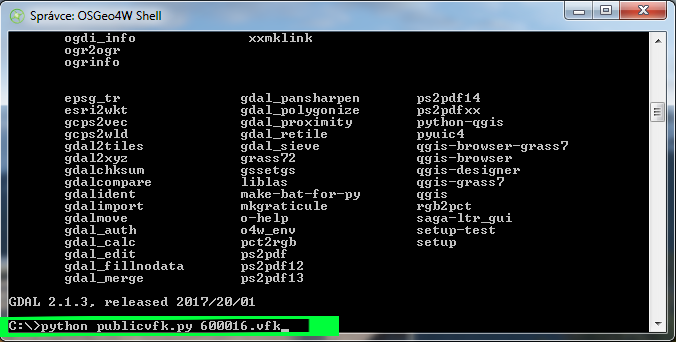
\includegraphics[height=7cm]{./pictures/testovani_ukazka.png}
      \caption{Ukázka testovacího spuštění knihovny}
      \label{fig:testovani_ukazka}
  \end{figure}

Zadání názvu knihovny i názvu \zk{VFK} souboru současně kontroluje
podmínka (\ref{lst:chyba}), pokud je spuštění knihovny nekorektní je
interpret ukončen a zobrazena chybová hláška
(obr. \ref{fig:testovani_hlaska}).
\begin{lstlisting}[caption=Podmínka pro spouštěcí příkaz, language=Python, label=lst:chyba, numbers=none]
    if len(sys.argv) != 2:
        sys.exit("{} soubor.vfk".format(sys.argv[0]))
\end{lstlisting}

\begin{figure}[H]
	 \centering
      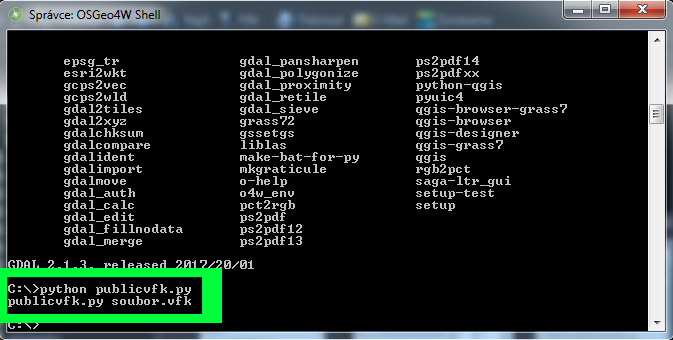
\includegraphics[height=7cm]{./pictures/testovani_hlaska.png}
      \caption{Chybová hláška včetně nekompletního příkazu při nesprávném použití knihovny}
      \label{fig:testovani_hlaska}
  \end{figure}

Testování je možné jen při přímém spuštění knihovny, nikoli je-li
knihovna importována jako modul. K tomu je využita speciální proměnná
\verb|__name__|, do které je interpretrem v případě spuštění přímo
uložena hodnota \verb|"__main__"| a podmínka je
splněna (viz.\ref{lst:podminka}). Je-li knihovna importována z jiného
modulu je proměnná \verb|__name__| nastavena na jméno modulu a
podmínka není splněna.
\begin{lstlisting}[caption=Ukázka sestavení bloků provedeném jen při přímém spuštění knihovny, language=Python, numbers=none, label=lst:podminka]
if __name__ == "__main__":
	#Sestaveni bloku primo z knihovny
    parcel = VFKParBuilder(sys.argv[1])
    parcel.build_all_par()
    building = VFKBudBuilder(sys.argv[1])
    building.build_all_bud()
\end{lstlisting}
%ucebnice jazyka Python str 10
